% One-page CV of Arno Rüegg.
% Build from this folder with:  latexmk -lualatex cv.tex
% (LuaLaTeX because the academicons ORCID icon needs a Unicode engine.)
% The website links assets/CV_Arno.pdf, so copy cv.pdf there when publishing.

\documentclass[10pt,a4paper]{article}

\usepackage[default]{sourcesanspro}
\usepackage[a4paper,top=1.1cm,bottom=1.0cm,left=1.4cm,right=1.4cm]{geometry}
\usepackage{xcolor}
\usepackage{graphicx}
\usepackage{tikz}
\usepackage{titlesec}
\usepackage{enumitem}
\usepackage{tabularx}
\usepackage{fontawesome5}
\usepackage{academicons}
\usepackage{accsupp}
\usepackage[hidelinks]{hyperref}

\graphicspath{{../assets/}}

% Colours taken from the website (style.css) so CV and site read as one brand.
\definecolor{ink}{HTML}{1D1C1A}
\definecolor{inksoft}{HTML}{4F4B44}
\definecolor{accent}{HTML}{A81B13}
\definecolor{rule}{HTML}{DDD6C6}

\color{ink}
\pagestyle{empty}
\setlength{\parindent}{0pt}
\setlength{\parskip}{0pt}
\linespread{1.04}
\raggedright
\frenchspacing

\hypersetup{
  pdftitle={CV Arno Rüegg},
  pdfauthor={Arno Rüegg},
}

% Section headings: small caps label in the accent colour with a thin rule.
\titleformat{\section}
  {\large\bfseries\color{accent}\scshape}
  {}{0pt}{}
  [\vspace{-0.55em}{\color{rule}\rule{\linewidth}{0.8pt}}]
\titlespacing*{\section}{0pt}{0.6em}{0.4em}

% Shared label width so the Skills and Leadership tables line up.
\newlength{\labelcolwidth}
\setlength{\labelcolwidth}{2.7cm}

\setlist[itemize]{leftmargin=1.1em, itemsep=0.1em, topsep=0.15em, parsep=0pt, label={\color{inksoft}\textbullet}}

% \cventry{title}{institution}{dates or venue}
% Everything sits on one line to keep the CV to one page; the body
% (bullets or text) follows the command directly.
\newcommand{\cventry}[3]{%
  \par\vspace{0.3em}%
  {\bfseries #1}\ifx\relax#2\relax\else, {\itshape #2}\fi\hfill{\color{inksoft}#3}\par
}

% \silenticon{icon}: icon glyphs otherwise come out as words like "GLOBE" when
% recruiting software extracts the PDF text, so their text is set to a space.
\newcommand{\silenticon}[1]{\BeginAccSupp{method=plain,ActualText={ }}#1\EndAccSupp{}}

% \linkedtitle{url}{title}: publication or thesis title that is clickable itself,
% followed by a small external-link icon as a visual cue that it is a link.
\newcommand{\linkedtitle}[2]{\href{#1}{#2}\,\href{#1}{{\color{accent}\scriptsize\silenticon{\faExternalLink*}}}}

% \contact{icon}{link target}{shown text}
\newcommand{\contact}[3]{\mbox{{\color{accent}\silenticon{#1}}\,\href{#2}{#3}}}

\begin{document}

% ---------- Header ----------
\begin{minipage}[c]{0.79\linewidth}
  {\fontsize{24}{28}\selectfont\bfseries Arno Rüegg}\par\vspace{0.25em}
  {\large\color{inksoft} Machine Learning Researcher · PhD candidate at ETH Zürich}\par\vspace{0.6em}
  \small
  \contact{\faEnvelope[regular]}{mailto:arno.rueegg@gmail.com}{arno.rueegg@gmail.com}\quad
  \contact{\faGlobe}{https://www.arnorueegg.ch/}{arnorueegg.ch}\quad
  \contact{\faLinkedin}{https://www.linkedin.com/in/arnorueegg}{linkedin.com/in/arnorueegg}\par\vspace{0.2em}
  \contact{\faGithub}{https://github.com/arrueegg}{github.com/arrueegg}\quad
  \contact{\aiOrcid}{https://orcid.org/0009-0004-7410-458X}{0009-0004-7410-458X}\quad
  \mbox{{\color{accent}\silenticon{\faBirthdayCake}}\,1 March 1999}
\end{minipage}%
\hfill
\begin{minipage}[c]{0.17\linewidth}
  \raggedleft
  \begin{tikzpicture}
    \clip (0,0) circle (1.25cm);
    \node at (0,0) {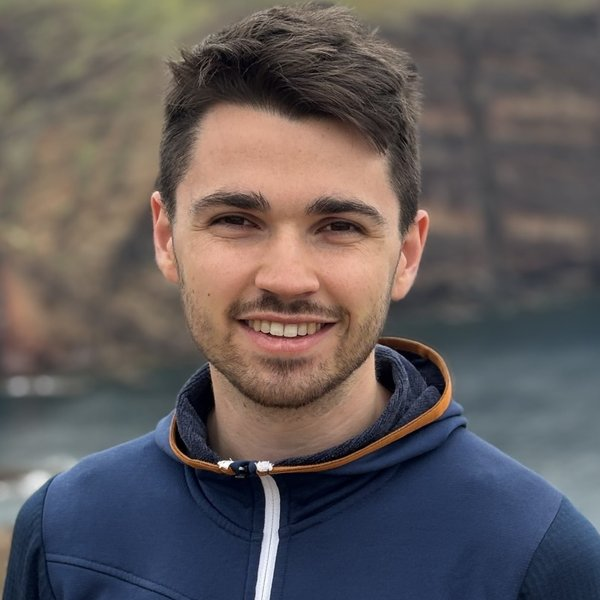
\includegraphics[width=2.5cm]{portrait.jpg}};
  \end{tikzpicture}
\end{minipage}

\vspace{0.7em}
{\small\color{inksoft}\silenticon{\faMapSigns}\enspace\textbf{Available from summer 2027} for applied ML roles in weather \& climate, remote sensing, GNSS and geospatial analytics.}

% ---------- Profile ----------
\section{Profile}
Machine-learning researcher who builds multi-modal models that fuse satellite and ground sensor data and know how uncertain they are.
Over three years of taking heterogeneous observations to validated transformer and probabilistic deep-learning models on GPU clusters;
four first-author papers, two of them peer-reviewed. Looking for applied problems where sensors are noisy and decisions need error bars.

% ---------- Research experience ----------
% The PhD is listed as a role because, for industry readers, it is four years of applied ML work.
\section{Research Experience}
\cventry{Doctoral Researcher}{ETH Zürich, Space Geodesy group}{2023 -- 2027 (expected)}
\begin{itemize}
  \item \textbf{Foundation model (Hemera).} Designing and training an 89M-parameter Perceiver-style transformer that fuses six observation types
        (GNSS, altimetry, radio occultation, ionosphere maps, space-weather indices) from 16 years into one latent global state;
        pretrained by predicting held-out observations, fine-tuned for 24\,h forecasting.
  \item \textbf{Probabilistic modelling.} Bayesian residual MLP with per-observation uncertainty, pretrained on 11 years of GNSS data:
        \textbf{24.5\% lower} single-frequency positioning error than the IGS maps, better on \textbf{96\%} of test days.
  \item \textbf{Multi-sensor data fusion.} Weighted-loss fusion of dense GNSS with sparse VLBI data:
        \textbf{about 50\% lower} median residuals near VLBI sites, validated on a year of independent Jason-3 altimetry.
  \item \textbf{Supervision.} Supervised \textbf{8 students} in four MSc projects and a BSc thesis (2024--2026), four of them on ML
        (GNNs, probabilistic networks, large-scale pretraining, LiDAR biomass mapping); a Data Science Lab team (ETH AI Center) I designed and supervised
        cut STEC test error by \textbf{22\%} over its baseline with large-scale pretraining and solar indices.
\end{itemize}

% ---------- Publications ----------
\section{Publications {\normalfont\small\color{inksoft}· all as first author}}
\begin{enumerate}[leftmargin=1.4em, itemsep=0.15em, topsep=0.1em, label={\color{inksoft}[\arabic*]}]
  \item Hemera: a Multi-Modal Foundation Model for the Global Ionospheric State. \hfill{\color{inksoft}\emph{in preparation}}
  \item \linkedtitle{https://essopenarchive.org/doi/full/10.22541/essoar.15003406/v1}{Probabilistic Machine Learning for Slant Total Electron Content Modelling based on GNSS.} \hfill{\color{inksoft}\emph{JGR: MLC, submitted}}
  \item \linkedtitle{https://link.springer.com/chapter/10.1007/1345_2026_315}{Fusion of GNSS and VLBI Data for Global Ionospheric Mapping.} \hfill{\color{inksoft}\emph{IAG Symposia (Springer), 2026}}
  \item \linkedtitle{https://agupubs.onlinelibrary.wiley.com/doi/10.1029/2025SW004540}{A Comparative Study of VTEC Estimates Derived from S/X VLBI and VGOS Observations.} \hfill{\color{inksoft}\emph{Space Weather (AGU), 2025}}
\end{enumerate}

% ---------- Education ----------
\section{Education}
\cventry{PhD in Space Geodesy}{ETH Zürich}{2023 -- 2027 (expected)}
\cventry{MSc Geomatics (Geoinformatics)}{ETH Zürich}{2021 -- 2023}
\begin{itemize}
  \item Thesis: \linkedtitle{https://ethz.ch/content/dam/ethz/special-interest/baug/igp/photogrammetry-remote-sensing-dam/documents/pdf/Student_Theses/2023/R\%C3\%BCegg_Arno_MSc_2023.pdf}{\emph{Shared Deep Feature Embedding of Sentinel-1 and Sentinel-2 for Building Detection}}.
        SAR--optical segmentation with adversarial domain alignment; \textbf{+3.1 pts IoU} from Stable Diffusion VAE features.
  \item Project: \linkedtitle{https://ethz.ch/content/dam/ethz/special-interest/baug/igp/photogrammetry-remote-sensing-dam/documents/pdf/Student_Theses/2022/IPA_ArnoR\%C3\%BCegg.pdf}{\emph{Vegetation Mapping with ICESat-2}}.
        Bias-corrected a canopy-height map: RMSE \textbf{7.6 $\to$ 6.0\,m} in seven regions.
\end{itemize}
\cventry{BSc Geospatial Engineering}{ETH Zürich}{2018 -- 2021}
\begin{itemize}
  \item Thesis: \linkedtitle{https://ethz.ch/content/dam/ethz/special-interest/baug/igp/photogrammetry-remote-sensing-dam/documents/pdf/Student_Theses/2021/R\%C3\%BCegg_Arno_BSc_2021.pdf}{\emph{Classification of Solid and Loose Rock on Orthophotos with Deep Learning}}.
        U-Net, \textbf{84.5\%} test accuracy.
\end{itemize}

% ---------- Skills ----------
\section{Skills}
\begin{tabularx}{\linewidth}{@{}>{\bfseries}p{\labelcolwidth} >{\raggedright\arraybackslash}X@{}}
  Machine learning & Foundation models, transformers, self-supervised pretraining, multi-modal data fusion, probabilistic deep learning, uncertainty quantification, spatiotemporal forecasting, computer vision \\[0.15em]
  Engineering      & Python, PyTorch (bf16 mixed precision), NumPy, pandas, SciPy, pytest, W\&B, Bash, Git, AI coding agents (Claude Code); basic C++, MATLAB, SQL \\[0.15em]
  Data \& compute  & xarray, Zarr, HDF5, netCDF, Parquet; Matplotlib, Cartopy; SLURM on ETH's Euler HPC cluster (A100 GPUs) \\[0.15em]
  Domain           & Ionosphere \& space weather, GNSS, VLBI, Earth observation, parameter estimation, photogrammetry \\
\end{tabularx}

% ---------- Leadership, languages and interests ----------
\section{Leadership \& More}
\begin{tabularx}{\linewidth}{@{}>{\bfseries}p{\labelcolwidth} >{\raggedright\arraybackslash}X r@{}}
  Leadership & Head of scout department, Pfadi Trogen: led four teams of 6--8 volunteer leaders & {\color{inksoft}2021 -- 2025} \\[0.15em]
  Teaching   & Teaching assistant: Geodetic Data Analysis, Measurement Techniques, Linear Algebra & {\color{inksoft}2021 -- 2026} \\[0.15em]
  Languages  & German (native), English (fluent), French (basic) & \\[0.15em]
  Interests  & Hiking, skiing, football, scouting & \\
\end{tabularx}

\end{document}
